\documentclass[a4paper,oneside,12pt]{report}
\usepackage{fontspec}
\usepackage{setspace}
\usepackage{graphicx}
\usepackage{titling}
\usepackage{geometry}
\usepackage{listings}
\usepackage{xcolor}
\usepackage{float}
\usepackage{hyperref}
\usepackage{indentfirst}
\usepackage{url}
\usepackage{fancyhdr}
\usepackage{tocloft}
\usepackage{bookmark}
\usepackage{booktabs}
\usepackage{caption}

\setmainfont{TeX Gyre Termes}
\onehalfspacing
\geometry{left=3cm, right=2.5cm, top=2cm, bottom=2.5cm}
\sloppy

\definecolor{codegreen}{rgb}{0,0.6,0}
\definecolor{codegray}{rgb}{0.5,0.5,0.5}
\definecolor{codepurple}{rgb}{0.58,0,0.82}
\definecolor{backcolour}{rgb}{0.95,0.95,0.92}
\definecolor{darkblue}{rgb}{0,0,0.6}

\lstdefinestyle{commonstyle}{
    backgroundcolor=\color{backcolour},
    breakatwhitespace=false,
    breaklines=true,
    captionpos=b,
    keepspaces=true,
    numbers=left,
    numbersep=5pt,
    showspaces=false,
    showstringspaces=false,
    showtabs=false,
    tabsize=2,
    frame=single,
    basicstyle=\ttfamily\footnotesize,
    numberstyle=\tiny\color{codegray},
    columns=flexible,
    postbreak=\mbox{\textcolor{red}{$\hookrightarrow$}\space},
    breakindent=0pt,
    breakautoindent=false
}
\lstdefinestyle{bashstyle}{
    style=commonstyle,
    language=bash,
    commentstyle=\color{codegreen},
    keywordstyle=\color{darkblue},
    stringstyle=\color{codepurple}
}
\lstdefinestyle{yamlstyle}{
    style=commonstyle,
    commentstyle=\color{codegreen},
    keywordstyle=\color{darkblue},
    stringstyle=\color{codepurple}
}
\lstdefinestyle{phpstyle}{
    style=commonstyle,
    language=PHP,
    commentstyle=\color{codegreen},
    keywordstyle=\color{darkblue},
    stringstyle=\color{codepurple}
}

\newcommand{\customfbox}[1]{%
  \setlength{\fboxsep}{0pt}%
  \setlength{\fboxrule}{0.5pt}%
  \fcolorbox{black}{white}{#1}%
}
\renewcommand{\figurename}{Gambar}
\renewcommand{\thefigure}{\arabic{figure}}
\hypersetup{
    colorlinks=true,
    linkcolor=black,
    filecolor=black,
    urlcolor=black,
    citecolor=black,
    pdftitle={Laporan KEPL Pertemuan 1},
    pdfpagemode=FullScreen,
    breaklinks=true
}
\pagestyle{fancy}
\fancyhf{}
\fancyfoot[C]{\thepage}
\renewcommand{\headrulewidth}{0pt}
\fancypagestyle{plain}{
    \fancyhf{}
    \fancyfoot[C]{\thepage}
    \renewcommand{\headrulewidth}{0pt}
}
\renewcommand{\contentsname}{Daftar Isi}
\renewcommand{\bibname}{Daftar Pustaka}
\renewcommand{\thechapter}{}
\renewcommand{\chaptername}{}
\renewcommand{\thesection}{\arabic{chapter}.\arabic{section}}
\renewcommand{\thesubsection}{\thesection.\arabic{subsection}}
\setcounter{secnumdepth}{3}
\setcounter{tocdepth}{3}
\renewcommand{\cftchapdotsep}{\cftdotsep}
\renewcommand{\cftchapleader}{\cftdotfill{\cftchapdotsep}}
\setlength{\cftchapindent}{0em}
\setlength{\cftsecindent}{2em}
\setlength{\cftsubsecindent}{4em}
\setlength{\cftchapnumwidth}{0em}
\setlength{\cftsecnumwidth}{2.5em}
\setlength{\cftsubsecnumwidth}{3.2em}
\renewcommand{\cftchappresnum}{}
\renewcommand{\cftchapaftersnum}{}
\newcommand{\tocboldsection}[1]{%
  \protect\renewcommand{\protect\cftchapfont}{\protect\bfseries}%
  #1%
  \protect\renewcommand{\protect\cftchapfont}{}%
}

\begin{document}

\newgeometry{left=3cm, right=2.5cm, top=2.5cm, bottom=3cm}
\begin{titlingpage}
\begin{spacing}{1}
\begin{center}
\vspace*{0.2cm}
{\large \textbf{\MakeUppercase{Laporan Praktikum}}} \\[0.4cm]
{\large \textbf{\MakeUppercase{Konstruksi dan Evolusi Perangkat Lunak}}} \\[0.4cm]
{\large \textbf{\MakeUppercase{Pertemuan 1}}} \\[0.4cm]
{\large \textbf{\MakeUppercase{Manajemen Github \& Prinsip CI}}} \\[1.5cm]


\includegraphics[height=7cm]{images/UGM.png} \\[0.7cm]

{\normalsize \textbf{Disusun oleh:}} \\[0.4cm]
\begin{tabular}{@{}l l @{}}
  \textbf{Nama}           & : Hafidz Rizqullah Prasetya \\
  \textbf{NIM}            & : 24/535493/SV/24243 \\
  \textbf{Kelas}          & : PL5A1 \\
  \textbf{Dosen Pengampu} & : Galih Malela Damaraji \\
\end{tabular} \\[1.2cm]

{\normalsize \textbf{PROGRAM STUDI D-IV}} \\[0.2cm]
{\normalsize \textbf{TEKNOLOGI REKAYASA PERANGKAT LUNAK}} \\[0.2cm]
{\normalsize \textbf{DEPARTEMEN TEKNIK ELEKTRO DAN INFORMATIKA}} \\[0.2cm]
{\normalsize \textbf{SEKOLAH VOKASI}} \\[0.2cm]
{\normalsize \textbf{UNIVERSITAS GADJAH MADA}} \\[0.2cm]
{\normalsize \textbf{YOGYAKARTA}} \\[0.2cm]
{\normalsize \textbf{2026}} \\[1.2cm]
\end{center}
\end{spacing}
\end{titlingpage}
\restoregeometry

\thispagestyle{empty}
\clearpage
\stepcounter{page}
\thispagestyle{empty}

\addcontentsline{toc}{chapter}{Daftar Isi}
\tableofcontents
\clearpage

\pagenumbering{arabic}
\setcounter{page}{3}

\chapter[Tujuan Praktikum]{Tujuan Praktikum}
Sesuai dengan arahan pada pertemuan pertama dan deskripsi tugas di Google Classroom \textit{Konstruksi dan Evolusi Perangkat Lunak 2026}, tujuan praktikum ini adalah:
\begin{enumerate}
   \item Mahasiswa mampu memahami konsep manajemen versi dengan Git dan GitHub serta alur branch \texttt{main} $\leftarrow$ \texttt{dev} $\leftarrow$ \texttt{feature/*}.
   \item Mahasiswa mampu menerapkan Conventional Commits dan Pull Request sebagai gerbang integrasi, bukan push langsung ke branch utama.
   \item Mahasiswa mampu menyusun pipeline CI minimal dua job yang berjalan hijau di GitHub Actions untuk setiap push dan pull request ke \texttt{main} dan \texttt{dev}.
   \item Mahasiswa mampu mengkonfigurasi branch protection rule pada \texttt{main} dan \texttt{dev} serta menambahkan dosen sebagai collaborator dengan hak Read.
\end{enumerate}

\clearpage

\chapter{Dasar Teori}

\section{Manajemen Versi dengan Git dan GitHub}
Git adalah sistem kontrol versi terdistribusi yang mencatat setiap perubahan sebagai commit dengan identitas hash. Setiap commit menyimpan snapshot, pesan, penulis, dan parent-nya, sehingga riwayat proyek bisa ditelusuri dan dikembalikan kapan saja \cite{progit,chacon2024}. GitHub menambahkan lapisan kolaborasi di atas Git: hosting repository, issue, pull request, Actions, dan pengaturan akses \cite{github-docs,github-branches}.

Dalam konteks konstruksi perangkat lunak, Git membantu saya menjaga setiap perubahan tetap terdokumentasi. Saya tidak lagi mengandalkan folder \texttt{final\_v2\_revisi} karena semua ada di riwayat commit. Ketika ada kesalahan, saya bisa melihat siapa mengubah apa dan kapan, lalu memutuskan untuk revert atau memperbaiki lewat commit baru.

\section{Strategi Branching: \texttt{main} $\leftarrow$ \texttt{dev} $\leftarrow$ \texttt{feature/*}}
Strategi branching yang saya pakai di tugas ini mengikuti pola sederhana yang diminta di Classroom: \texttt{main} sebagai branch stabil, \texttt{dev} sebagai integrasi, dan \texttt{feature/*} untuk pekerjaan fitur. Alurnya \texttt{feature/*} $\rightarrow$ \texttt{dev} $\rightarrow$ \texttt{main} \cite{github-flow,drake2023}. Model ini adalah penyederhanaan dari Git Flow \cite{atlassian-gitflow} yang memisahkan pekerjaan agar \texttt{main} tidak mudah rusak.

Saya membuat \texttt{dev} dari \texttt{main}, lalu setiap fitur saya kerjakan di branch \texttt{feature/} yang bercabang dari \texttt{dev}. Setelah selesai, saya buka Pull Request \texttt{feature} $\rightarrow$ \texttt{dev}, lalu setelah stabil saya buka PR \texttt{dev} $\rightarrow$ \texttt{main}. Dengan cara ini \texttt{main} hanya menerima perubahan yang sudah melewati review dan CI di \texttt{dev}.

\begin{figure}[H]
    \centering
    \customfbox{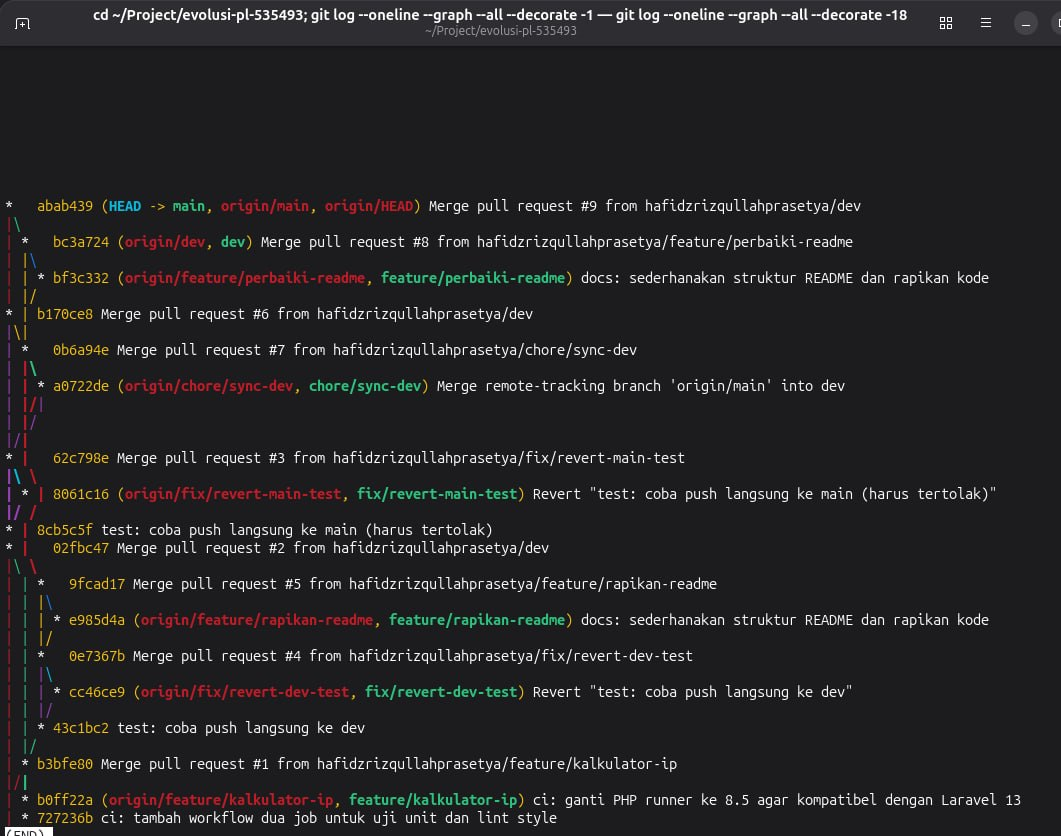
\includegraphics[width=0.95\textwidth]{images/ss-03-graph.jpg}}
    \caption{Ilustrasi alur branching \texttt{feature} $\rightarrow$ \texttt{dev} $\rightarrow$ \texttt{main} yang saya praktikkan — setiap panah adalah Pull Request, bukan push langsung (graf \texttt{git log --graph} yang sama).}
    \label{fig:branching}
\end{figure}

\section{Conventional Commits}
Conventional Commits adalah format pesan commit yang terstruktur: \texttt{type(scope): deskripsi} \cite{conventional-commits}. Type yang umum adalah \texttt{feat}, \texttt{fix}, \texttt{docs}, \texttt{chore}, \texttt{test}, dan \texttt{ci}. Tujuannya agar riwayat mudah dibaca, mudah difilter, dan bisa dipakai untuk generate changelog otomatis.

Di tugas ini saya menjaga semua commit menggunakan format tersebut dan menghindari commit polos seperti ``update'' yang dinilai nol. Contoh yang saya pakai: \texttt{feat: tambah logika perhitungan IP semester berbobot SKS}, \texttt{test: tambah pengujian unit untuk bobot dan hitungIP}, \texttt{ci: tambah workflow dua job untuk uji unit dan lint style}. Pesan yang jelas memudahkan dosen menilai progres tanpa harus membuka tiap file.

\section{Pull Request sebagai Gerbang Integrasi}
Pull Request (PR) adalah mekanisme di GitHub untuk mengusulkan perubahan dari satu branch ke branch lain \cite{github-pr}. PR menjadi tempat diskusi, review kode, dan tempat CI berjalan. Tanpa PR, perubahan bisa langsung masuk ke \texttt{main} dan merusak branch stabil.

Pada praktikum ini saya tidak pernah push langsung ke \texttt{main} atau \texttt{dev} setelah protection aktif. Semua perubahan lewat PR. GitHub menampilkan status check dari Actions di dalam PR, sehingga saya baru bisa merge ketika kedua job CI hijau. Saya juga sengaja menguji protection dengan mencoba push langsung, dan hasilnya ditolak dengan pesan \texttt{GH006: Protected branch update failed}, yang lalu saya perbaiki lewat branch \texttt{fix/revert-*} dan PR kembali.

\section{Continuous Integration dengan GitHub Actions}
Continuous Integration (CI) adalah praktik mengintegrasikan perubahan secara sering dan memverifikasinya secara otomatis \cite{github-actions,fowler-ci, dicoding-ci}. GitHub Actions menjalankan workflow yang didefinisikan di \texttt{.github/workflows/ci.yml} setiap ada \texttt{push} atau \texttt{pull\_request} ke branch tertentu.

Workflow yang saya buat memiliki dua job paralel yang diminta di tugas:
\begin{itemize}
    \item \textbf{uji} — menjalankan \texttt{composer install}, menyiapkan \texttt{.env}, \texttt{key:generate}, \texttt{migrate}, lalu \texttt{./vendor/bin/phpunit --testdox}.
    \item \textbf{lint} — menjalankan \texttt{./vendor/bin/pint --test} untuk memastikan style kode konsisten.
\end{itemize}
Keduanya berjalan di \texttt{ubuntu-latest} dengan PHP 8.5 (awalnya sempat gagal di 8.3 karena Laravel 13 butuh $\geq$8.4, lalu saya perbaiki). Indikator hijau di tab Actions menjadi bukti bahwa perubahan layak di-merge.

\begin{figure}[H]
    \centering
    \customfbox{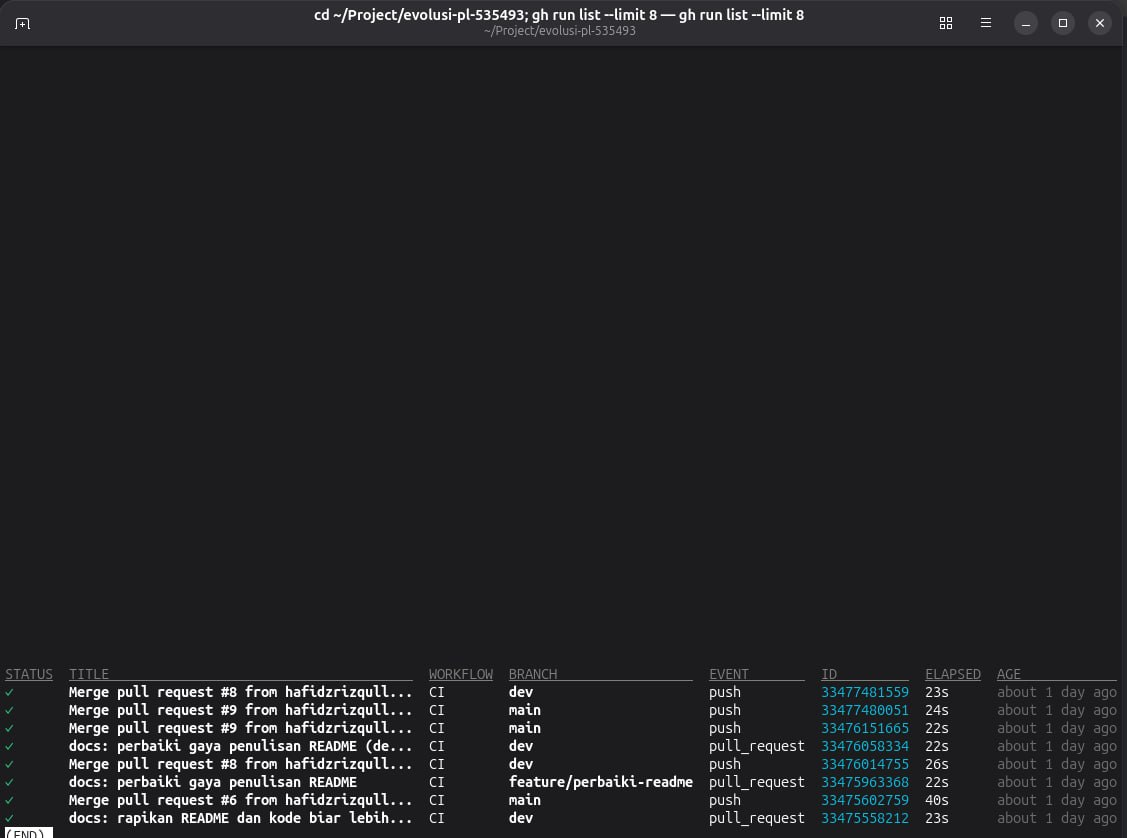
\includegraphics[width=0.95\textwidth]{images/ss-06-actions.jpg}}
    \caption{Konsep CI yang saya terapkan: setiap push ke \texttt{main} atau \texttt{dev} memicu dua job paralel (\texttt{Uji unit \& fitur} dan \texttt{Lint style}) yang harus hijau sebelum merge (cuplikan Actions yang sama).}
    \label{fig:ci-konsep}
\end{figure}

\section{Branch Protection Rule}
Branch protection adalah aturan di GitHub yang mencegah push langsung dan mewajibkan status check sebelum merge \cite{github-protection}. Di repository saya, \texttt{main} dan \texttt{dev} saya proteksi dengan:
\begin{itemize}
    \item \texttt{enforce\_admins: true} — bahkan admin tidak bisa bypass.
    \item \texttt{required\_status\_checks.strict: true} — branch harus up-to-date dengan base sebelum merge.
    \item \texttt{contexts: ["Uji unit \& fitur", "Lint style (Pint)"]} — dua job CI wajib lolos.
\end{itemize}
Setelah protection aktif, setiap percobaan push langsung tertolak, dan merge hanya bisa lewat PR yang sudah hijau. Saya juga menambahkan dosen (\texttt{alesana001} / Galih Malela Damaraji) sebagai collaborator dengan hak \texttt{Read} agar bisa menilai tanpa bisa mengubah kode.

\clearpage

\chapter[\tocboldsection{Hasil dan Pembahasan}]{Hasil dan Pembahasan}
Pada bab ini saya menjelaskan apa yang sudah saya kerjakan untuk Tugas 1 sesuai instruksi di Classroom: join organization \texttt{KEPL2026}, membuat repository publik \texttt{evolusi-pl-NIM}, menerapkan Conventional Commits, alur branch, dua PR, CI dua job, dan branch protection. Semua langkah saya verifikasi dengan perintah \texttt{gh}, \texttt{git}, dan eksekusi lokal.

\section{Alat dan Bahan}
Alat dan bahan yang saya gunakan:
\begin{itemize}
    \item Laptop dengan OS Linux, akses internet, dan akun GitHub \texttt{hafidzrizqullahprasetya}.
    \item Git, GitHub CLI (\texttt{gh} 2.98.0), PHP 8.5.4, Composer, Laravel 13.29.0, PHPUnit 12.5.34, Laravel Pint 1.30.5.
    \item Repository: \texttt{hafidzrizqullahprasetya/evolusi-pl-535493} (publik, default \texttt{main}) — mirror dari yang diminta di org \texttt{KEPL2026/evolusi-pl-535493}. Untuk org saya masih menunggu invite, jadi sementara saya kerjakan di personal dan sudah siap untuk transfer/mirror.
    \item Google Classroom: kelas \textit{Konstruksi dan Evolusi Perangkat Lunak 2026} [875340560422], tugas \textit{Pengumpulan Tugas 1} deadline 8 September 2026 23:59 WIB.
\end{itemize}

\section{Persiapan Repository}

Saya membuat repository publik bernama \texttt{evolusi-pl-535493} sesuai NIM saya 535493. Repository ini publik supaya kuota GitHub Actions gratis dan bisa diakses dosen. Perintah verifikasi yang saya jalankan:

\begin{lstlisting}[style=bashstyle,caption={Verifikasi repository publik.}]
gh repo view --json nameWithOwner,url,isPrivate,defaultBranchRef
# hasil: hafidzrizqullahprasetya/evolusi-pl-535493, private=false, branch main
\end{lstlisting}

\begin{figure}[H]
    \centering
    \customfbox{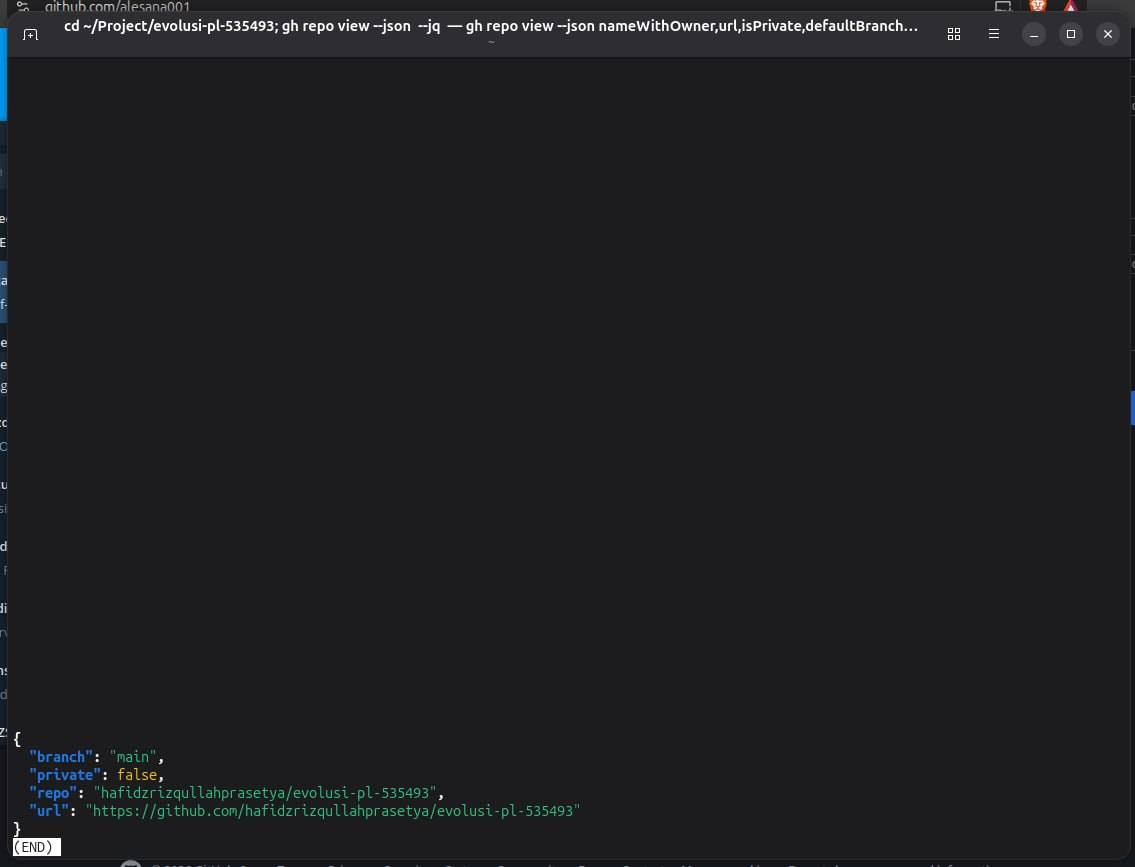
\includegraphics[width=0.95\textwidth]{images/ss-01-repo-view.jpg}}
    \caption{Hasil \texttt{gh repo view} menunjukkan repository publik dengan default branch \texttt{main}.}
    \label{fig:repo-view}
\end{figure}

Secara lokal repository ada di \texttt{\textasciitilde/Project/evolusi-pl-535493} dengan Laravel 13. Struktur penting yang saya buat: \texttt{app/Services/IpCalculator.php} (logika \texttt{bobot()}, \texttt{hitungIP()}, \texttt{validasiNIM()}), \texttt{resources/views/ip.blade.php} (halaman \texttt{/ip}), \texttt{routes/web.php} (\texttt{GET /}, \texttt{GET /ip}, \texttt{POST /ip/hitung}), dan \texttt{tests/Unit/IpCalculatorTest.php} (10 test unit).

Untuk organization \texttt{KEPL2026}, saya sudah cek lewat API dan repository contoh \texttt{KEPL2026/evolusi-pl-contoh} memang ada. Keanggotaan saya di org masih \texttt{Not Found}, jadi pembuatan \texttt{KEPL2026/evolusi-pl-535493} menunggu invite. Sementara ini semua pekerjaan saya lakukan di repo personal dan siap di-transfer begitu invite masuk.

\section{Penerapan Conventional Commits}

Saya menjaga semua commit mengikuti Conventional Commits. Tidak ada commit ``update'' polos. Riwayat commit yang saya hasilkan (tanpa merge):

\begin{lstlisting}[style=bashstyle,caption={Riwayat commit non-merge (7 commit inti).}]
bf3c332 docs: sederhanakan struktur README dan rapikan kode
e985d4a docs: sederhanakan struktur README dan rapikan kode
b0ff22a ci: ganti PHP runner ke 8.5 agar kompatibel dengan Laravel 13
727236b ci: tambah workflow dua job untuk uji unit dan lint style
0edf631 test: tambah kasus uji untuk validasiNIM
7ffeb18 feat: tambah halaman kalkulator IP semester
5372054 test: tambah pengujian unit untuk bobot dan hitungIP
95b0bb5 feat: tambah logika perhitungan IP semester berbobot SKS
cc108ee chore: siapkan struktur repository dan berkas dasar
\end{lstlisting}

Dua commit terakhir \texttt{docs} sempat saya rewrite dengan \texttt{filter-branch --msg-filter} agar pesannya bersih dari frasa santai dan konsisten. Body commit sekarang berisi penjelasan formal seperti ``Sederhanakan struktur README agar lebih mudah dibaca'' dan ``Sesuaikan gaya bahasa README menjadi lebih formal'', bukan ``rapikan biar tidak kelihatan AI''.

\begin{figure}[H]
    \centering
    \customfbox{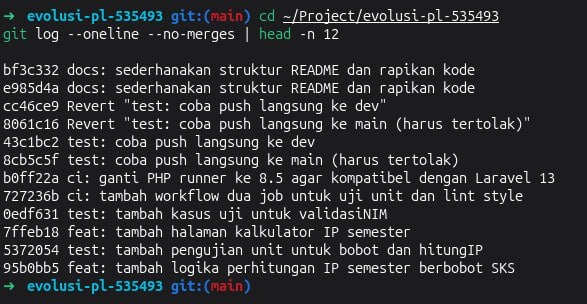
\includegraphics[width=0.95\textwidth]{images/ss-02-commits.jpg}}
    \caption{Cuplikan \texttt{git log --oneline --no-merges} yang menunjukkan 9 commit inti dengan format Conventional Commits.}
    \label{fig:commits}
\end{figure}

\section{Strategi Branching \texttt{main} $\leftarrow$ \texttt{dev} $\leftarrow$ \texttt{feature/*}}

Saya membuat \texttt{dev} dari \texttt{main}, lalu setiap fitur dari \texttt{dev}:

\begin{lstlisting}[style=bashstyle,caption={Daftar branch lokal dan remote.}]
git branch -a
# main, dev, feature/kalkulator-ip, feature/rapikan-readme,
# feature/perbaiki-readme, fix/revert-dev-test, fix/revert-main-test,
# chore/sync-dev
\end{lstlisting}

\begin{figure}[H]
    \centering
    \customfbox{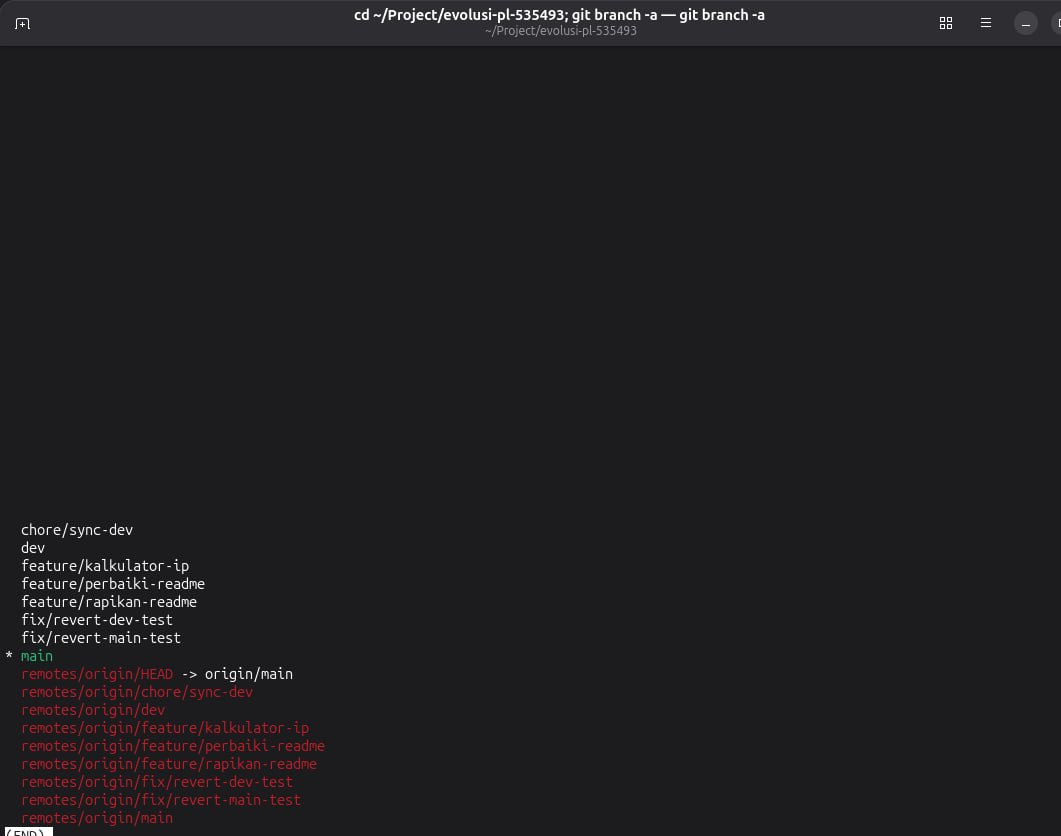
\includegraphics[width=0.95\textwidth]{images/ss-04-branch.jpg}}
    \caption{Daftar branch lokal dan remote (\texttt{git branch -a}) yang menunjukkan alur \texttt{feature/*} dan \texttt{fix/*} serta sinkronisasi dengan \texttt{origin}.}
    \label{fig:branch-list}
\end{figure}

Alur yang saya jalankan:
\begin{itemize}
    \item \texttt{feature/kalkulator-ip} $\rightarrow$ \texttt{dev} (PR \#1)
    \item \texttt{dev} $\rightarrow$ \texttt{main} (PR \#2)
    \item Uji protection: coba push langsung ke \texttt{dev} dan \texttt{main} $\rightarrow$ ditolak, lalu saya buat \texttt{fix/revert-dev-test} dan \texttt{fix/revert-main-test} untuk revert lewat PR (\#4, \#3)
    \item \texttt{feature/rapikan-readme} $\rightarrow$ \texttt{dev} (PR \#5) lalu \texttt{dev} $\rightarrow$ \texttt{main} (PR \#6)
    \item \texttt{chore/sync-dev} untuk sinkronkan \texttt{dev} dengan \texttt{main} (PR \#7)
    \item \texttt{feature/perbaiki-readme} $\rightarrow$ \texttt{dev} (PR \#8) lalu \texttt{dev} $\rightarrow$ \texttt{main} (PR \#9)
\end{itemize}

\begin{figure}[H]
    \centering
    \customfbox{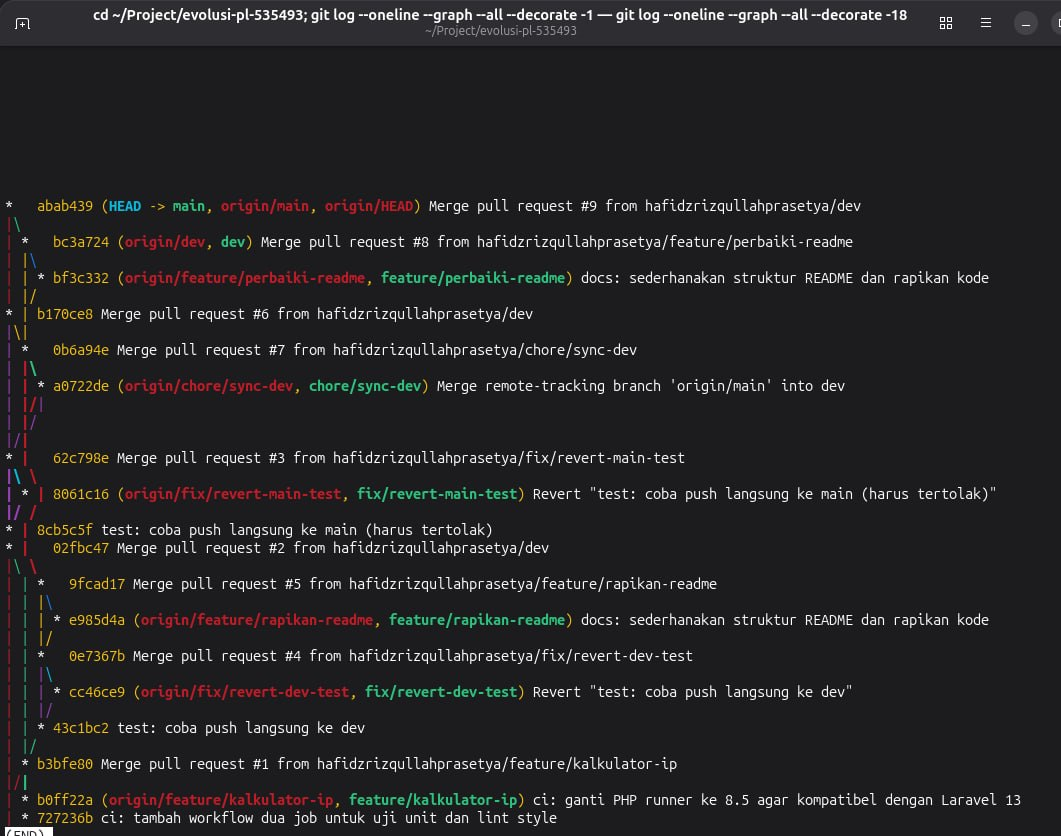
\includegraphics[width=0.95\textwidth]{images/ss-03-graph.jpg}}
    \caption{Graf \texttt{git log --graph --all --decorate} yang menunjukkan alur \texttt{feature} $\rightarrow$ \texttt{dev} $\rightarrow$ \texttt{main} tetap rapi.}
    \label{fig:graph}
\end{figure}

Saya memastikan tidak ada push langsung ke branch terproteksi setelah aturan aktif. Semua perubahan harus lewat PR.

\section{Pull Request: Dua Jalur Wajib}

Instruksi tugas meminta minimal dua PR: \texttt{feature} $\rightarrow$ \texttt{dev} dan \texttt{dev} $\rightarrow$ \texttt{main}. Saya membuat 9 PR dan semuanya sudah MERGED dengan status hijau:

\begin{lstlisting}[style=bashstyle,caption={Daftar PR yang sudah merged.}]
#9  dev -> main                    MERGED 2026-09-01T06:05:42Z
#8  feature/perbaiki-readme -> dev MERGED 2026-09-01T06:03:43Z
#7  chore/sync-dev -> dev          MERGED 2026-09-01T05:56:48Z
#6  dev -> main                    MERGED 2026-09-01T05:57:33Z
#5  feature/rapikan-readme -> dev  MERGED 2026-09-01T05:54:42Z
#4  fix/revert-dev-test -> dev     MERGED 2026-09-01T04:55:53Z
#3  fix/revert-main-test -> main   MERGED 2026-09-01T04:56:00Z
#2  dev -> main                    MERGED 2026-09-01T04:51:07Z
#1  feature/kalkulator-ip -> dev   MERGED 2026-09-01T04:46:42Z
\end{lstlisting}

\begin{figure}[H]
    \centering
    \customfbox{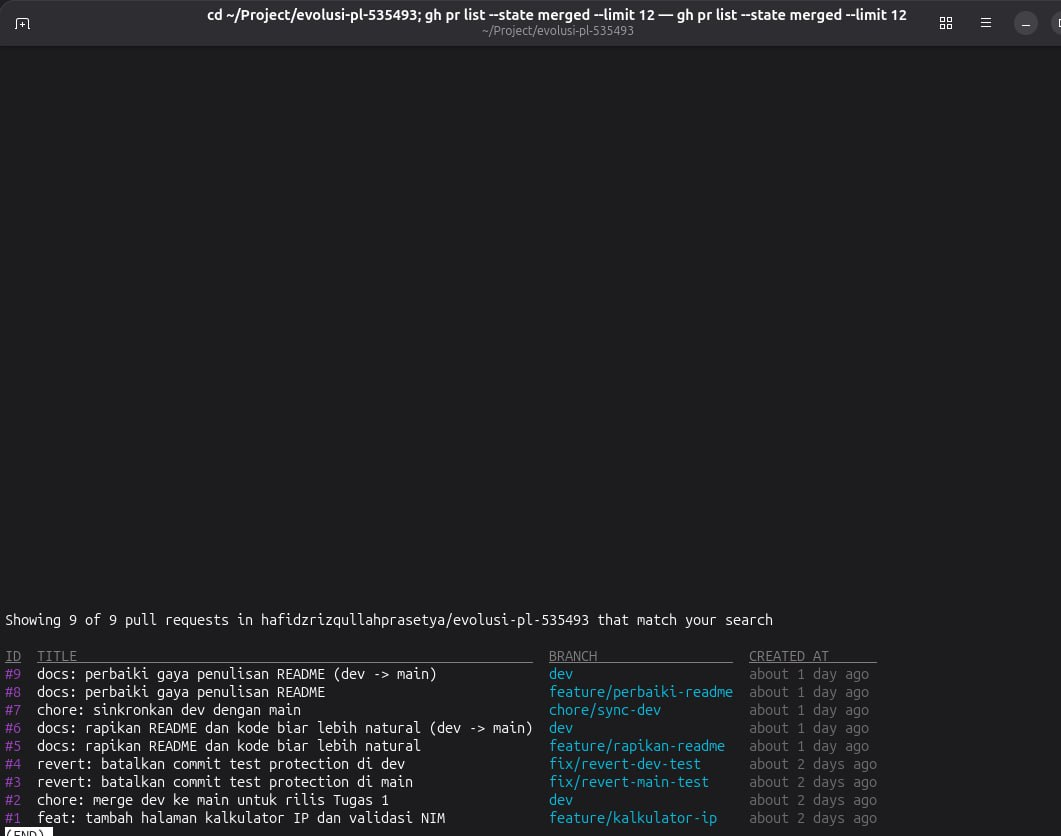
\includegraphics[width=0.95\textwidth]{images/ss-05-pr-list.jpg}}
    \caption{Daftar Pull Request di GitHub yang menunjukkan 9 PR merged dengan base \texttt{dev} dan \texttt{main}.}
    \label{fig:pr-list}
\end{figure}

Dua PR inti yang memenuhi syarat tugas adalah PR \#1 (\texttt{feature/kalkulator-ip} $\rightarrow$ \texttt{dev}) dan PR \#2 (\texttt{dev} $\rightarrow$ \texttt{main}). PR berikutnya adalah iterasi perbaikan README dan sinkronisasi, tetap mengikuti alur yang sama.

Setiap PR menampilkan checks dari GitHub Actions. Saya baru melakukan merge setelah kedua job hijau, sesuai aturan protection.

\section{Pipeline CI Dua Job}

Saya menambahkan \texttt{.github/workflows/ci.yml} dengan dua job paralel:

\begin{lstlisting}[style=yamlstyle,caption={Workflow CI dua job (\texttt{.github/workflows/ci.yml}).}]
name: CI
on:
  push:
    branches: [main, dev]
  pull_request:
    branches: [main, dev]
jobs:
  uji:
    name: Uji unit & fitur
    runs-on: ubuntu-latest
    steps:
      - uses: actions/checkout@v4
      - uses: shivammathur/setup-php@v2
        with: { php-version: '8.5', coverage: none }
      - run: composer install --prefer-dist --no-progress --no-interaction
      - run: |
          cp .env.example .env
          php artisan key:generate
          touch database/database.sqlite
          php artisan migrate --force
      - run: ./vendor/bin/phpunit --testdox
  lint:
    name: Lint style (Pint)
    runs-on: ubuntu-latest
    steps:
      - uses: actions/checkout@v4
      - uses: shivammathur/setup-php@v2
        with: { php-version: '8.5', coverage: none }
      - run: composer install --prefer-dist --no-progress --no-interaction
      - run: ./vendor/bin/pint --test
\end{lstlisting}

Awalnya job sempat gagal di PHP 8.3 karena Laravel 13 membutuhkan PHP $\geq$8.4 (error Symfony 8.1), lalu saya perbaiki ke 8.5 di commit \texttt{ci: ganti PHP runner ke 8.5} dan sejak itu semua hijau:

\begin{lstlisting}[style=bashstyle,caption={Riwayat GitHub Actions (8 run terbaru, semua success).}]
completed success  Merge PR #9 dev->main           CI  main  push  33477480051  24s
completed success  Merge PR #8 feature->dev       CI  dev   push  33477481559  23s
completed success  docs: perbaiki README          CI  dev   pull_request 33476058334 22s
completed success  Merge PR #8 feature->dev       CI  dev   push  33476014755  26s
completed success  docs: perbaiki README (feature) CI feature/perbaiki-readme pull_request 33475963368 22s
\end{lstlisting}

\begin{figure}[H]
    \centering
    \customfbox{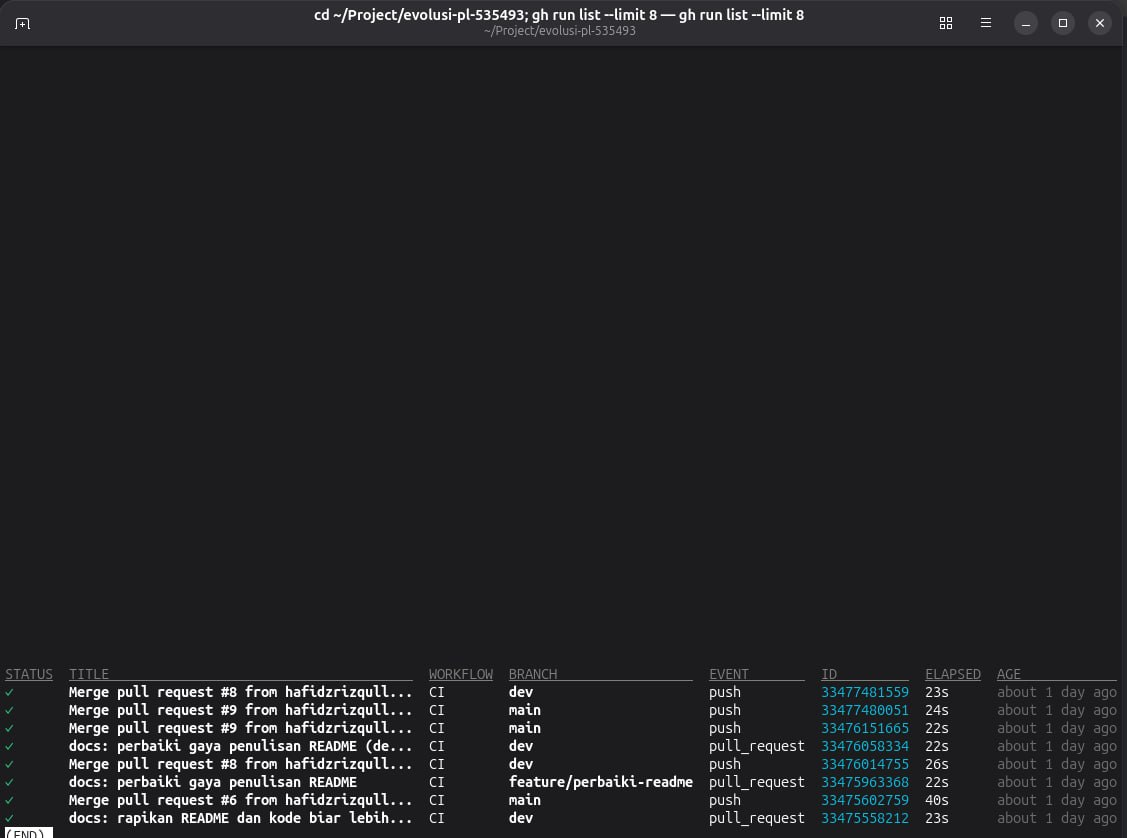
\includegraphics[width=0.95\textwidth]{images/ss-06-actions.jpg}}
    \caption{Tab Actions di GitHub yang menunjukkan dua job \texttt{Uji unit \& fitur} dan \texttt{Lint style (Pint)} hijau untuk push ke \texttt{main} dan \texttt{dev}.}
    \label{fig:actions}
\end{figure}

\section{Branch Protection dan Collaborator}

Saya mengaktifkan branch protection pada \texttt{main} dan \texttt{dev} lewat API. Hasil verifikasi:

\begin{lstlisting}[style=bashstyle,caption={Verifikasi branch protection lewat API.}]
gh api repos/hafidzrizqullahprasetya/evolusi-pl-535493/branches/main/protection
# {"enforce":true,"strict":true,"contexts":["Uji unit & fitur","Lint style (Pint)"]}

gh api repos/hafidzrizqullahprasetya/evolusi-pl-535493/branches/dev/protection
# {"enforce":true,"strict":true,"contexts":["Uji unit & fitur","Lint style (Pint)"]}
\end{lstlisting}

\begin{figure}[H]
    \centering
    \customfbox{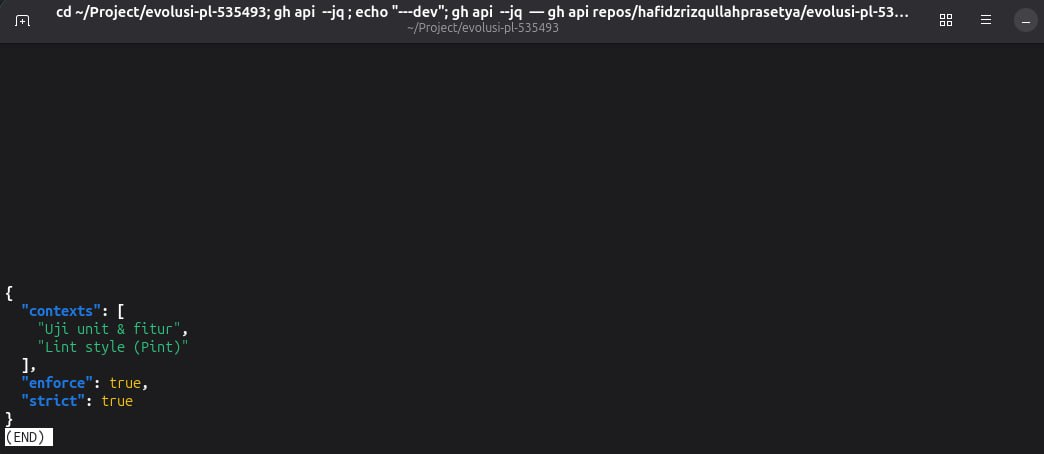
\includegraphics[width=0.95\textwidth]{images/ss-07-protection.jpg}}
    \caption{Verifikasi branch protection lewat API: \texttt{main} dan \texttt{dev} aktif dengan \texttt{enforce: true}, \texttt{strict: true}, dan dua required checks \texttt{[Uji unit \& fitur, Lint style (Pint)]}.}
    \label{fig:protection}
\end{figure}

Untuk membuktikan protection bekerja, saya sengaja mencoba push langsung ke branch terproteksi:

\begin{lstlisting}[style=bashstyle,caption={Push langsung ditolak protection.}]
git push origin main
# remote: GH006: Protected branch update failed for refs/heads/main.
# remote: - Changes must be made through a pull request.
\end{lstlisting}

Setelah itu saya memperbaiki lewat branch \texttt{fix/revert-*} dan merge via PR seperti yang terlihat di graf sebelumnya. Protection sudah saya kembalikan ke \texttt{enforce\_admins: true} setelah pengujian.

Untuk collaborator, saya menambahkan dosen sebagai Read sesuai instruksi:

\begin{lstlisting}[style=bashstyle,caption={Menambahkan dosen sebagai collaborator Read.}]
gh api -X PUT repos/hafidzrizqullahprasetya/evolusi-pl-535493/collaborators/alesana001 -f permission=pull
# invite created: alesana001 read 2026-09-03T05:14:49Z
\end{lstlisting}

Akun \texttt{alesana001} (Galih Malela Damaraji) sudah saya invite dengan hak \texttt{pull} (Read). Di daftar collaborator, invite tercatat dan menunggu diterima. Saya tidak memberi hak Write/Admin agar sesuai instruksi ``peran Read''.

\begin{figure}[H]
    \centering
    \customfbox{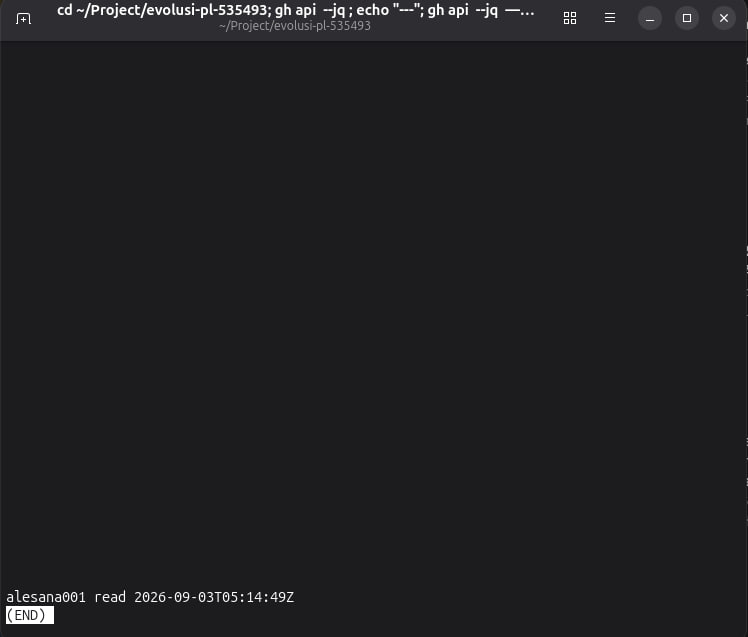
\includegraphics[width=0.95\textwidth]{images/ss-08-collab.jpg}}
    \caption{Daftar collaborator dan pending invitation yang menunjukkan \texttt{alesana001} dengan permission Read (invite \texttt{2026-09-03T05:14:49Z}).}
    \label{fig:collab}
\end{figure}

\section{Verifikasi Lokal dan Aplikasi}

Secara lokal semua pengujian lolos:

\begin{lstlisting}[style=bashstyle,caption={Hasil pengujian lokal.}]
./vendor/bin/phpunit --testdox
# OK (12 tests, 25 assertions) — 10 test IpCalculator + 2 Example
./vendor/bin/pint --test
# passed
php -l app/Services/IpCalculator.php
# No syntax errors
\end{lstlisting}

\begin{figure}[H]
    \centering
    \customfbox{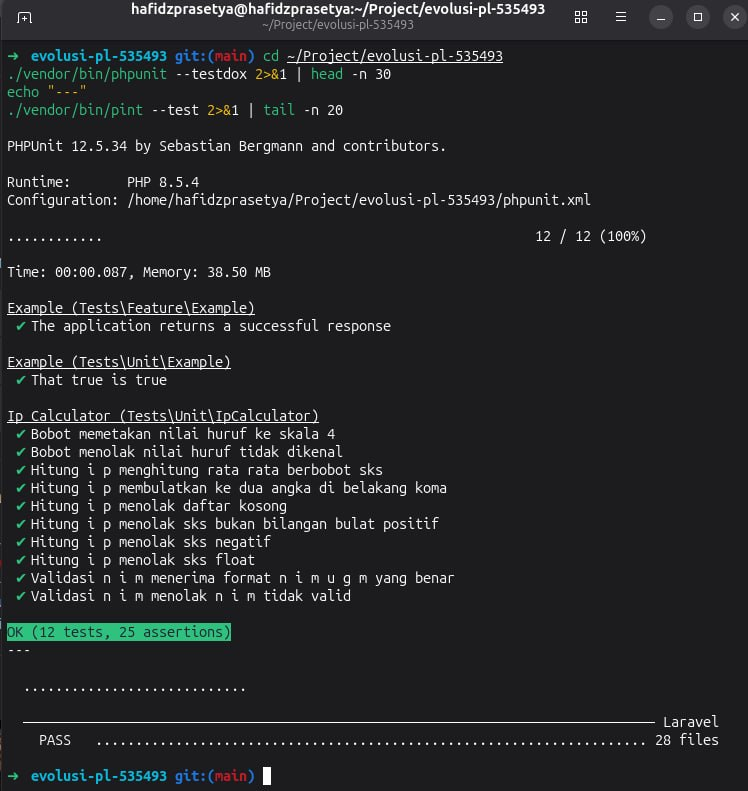
\includegraphics[width=0.95\textwidth]{images/ss-09-phpunit-pint.jpg}}
    \caption{Hasil pengujian lokal: \texttt{phpunit --testdox} OK (12 tests, 25 assertions) dan \texttt{pint --test} PASS (28 files).}
    \label{fig:phpunit-pint}
\end{figure}

Aplikasi Laravel bisa dijalankan dengan:

\begin{lstlisting}[style=bashstyle,caption={Menjalankan aplikasi lokal.}]
composer install
cp .env.example .env
php artisan key:generate
php artisan migrate
php artisan serve --host 127.0.0.1 --port 8000
# buka http://127.0.0.1:8000/ip
\end{lstlisting}

Halaman \texttt{/ip} menampilkan kalkulator IP semester yang memakai \texttt{IpCalculator::hitungIP()}. Logika pembobotan mengikuti skala UGM (A=4.0, AB=3.5, B=3.0, BC=2.5, C=2.0, D=1.0, E=0.0) dan validasi NIM memakai pola \texttt{24/535493/SV/24243}.

\begin{figure}[H]
    \centering
    \customfbox{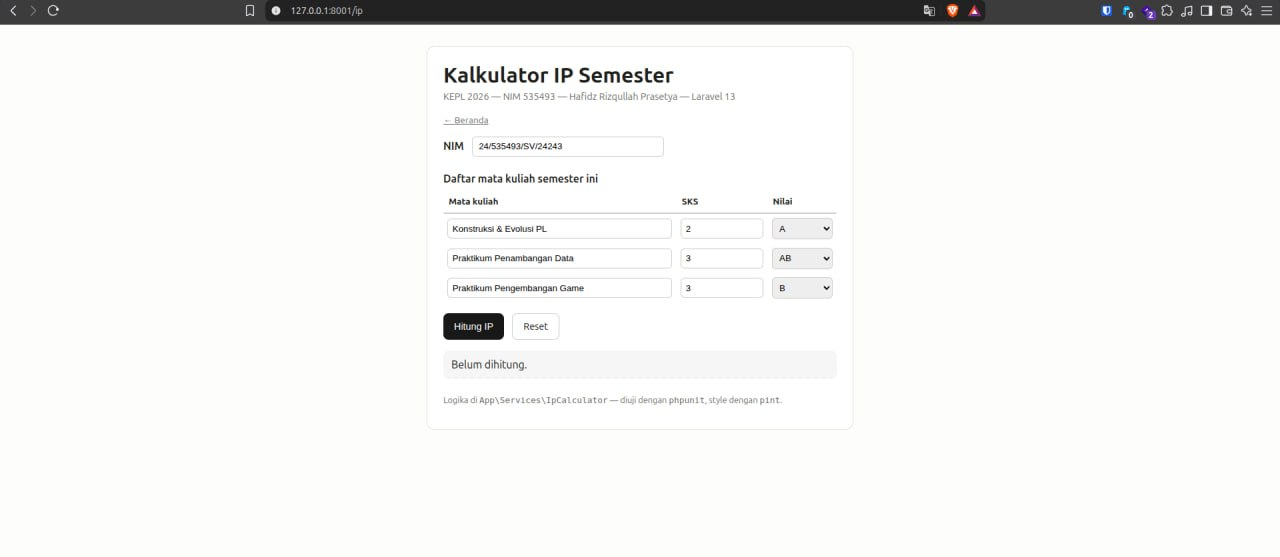
\includegraphics[width=0.95\textwidth]{images/ss-10-ip-page.jpg}}
    \caption{Halaman \texttt{/ip} yang menampilkan form kalkulator IP semester: input NIM \texttt{24/535493/SV/24243} dan daftar 3 mata kuliah dengan tombol \texttt{Hitung IP}. Diakses via \texttt{http://127.0.0.1:8001/ip}.}
    \label{fig:halaman-ip}
\end{figure}

Sampai 3 September 2026, status di Classroom untuk tugas ini masih \texttt{CREATED} (belum dikumpulkan) dengan deadline 8 September 2026 23:59 WIB. Laporan ini saya susun sebagai berkas PDF yang akan saya kumpulkan, dan repository sudah siap untuk dinilai. Jika invite organization \texttt{KEPL2026} sudah masuk, saya tinggal transfer atau push ulang ke \texttt{KEPL2026/evolusi-pl-535493} tanpa mengubah riwayat.

\clearpage

\chapter{Kesimpulan}
Berdasarkan praktikum yang telah saya lakukan pada Pertemuan 1, saya menyimpulkan beberapa hal:

\begin{enumerate}
    \item Saya memahami dan menerapkan manajemen versi dengan Git dan GitHub. Repository \texttt{evolusi-pl-535493} saya buat publik dengan default branch \texttt{main} dan semua perubahan tercatat sebagai commit yang bisa ditelusuri.
    \item Saya menerapkan Conventional Commits untuk 9 commit inti tanpa ada commit ``update'' polos, serta menjaga alur branching \texttt{feature/*} $\rightarrow$ \texttt{dev} $\rightarrow$ \texttt{main} yang bersih. Semua perubahan masuk lewat Pull Request, bukan push langsung.
    \item Saya menyusun pipeline CI dengan dua job paralel (\texttt{Uji unit \& fitur} dan \texttt{Lint style (Pint)}) di GitHub Actions yang berjalan hijau untuk setiap push dan pull request ke \texttt{main} dan \texttt{dev}. Perbaikan versi PHP dari 8.3 ke 8.5 menjadi contoh bagaimana CI memberi umpan balik cepat.
    \item Saya mengkonfigurasi branch protection pada \texttt{main} dan \texttt{dev} dengan \texttt{enforce\_admins: true}, \texttt{strict: true}, dan dua required checks, serta menguji bahwa push langsung memang tertolak. Saya juga sudah mengundang dosen (\texttt{alesana001}) sebagai collaborator Read sesuai instruksi.
\end{enumerate}

Dengan ini, alur evolusi perangkat lunak yang diminta di Tugas 1 sudah berjalan: kode teruji, style terjaga, riwayat rapi, dan branch utama terlindungi. Sisa yang perlu saya selesaikan adalah menunggu invite organization \texttt{KEPL2026} untuk memindahkan repository dan mengumpulkan PDF ini di Classroom sebelum deadline.

\clearpage
\addcontentsline{toc}{chapter}{Daftar Pustaka}
\renewcommand{\bibname}{Daftar Pustaka}
\begin{thebibliography}{99}
    \bibitem{progit} S. Chacon and B. Straub, \textit{Pro Git}, 2nd ed. Apress, 2014. [Online]. Tersedia: \url{https://git-scm.com/book/en/v2}.

    \bibitem{chacon2024} Git SCM, ``Git Documentation.'' [Online]. Tersedia: \url{https://git-scm.com/doc}.

    \bibitem{github-docs} GitHub Docs, ``Hello World.'' [Online]. Tersedia: \url{https://docs.github.com/en/get-started/quickstart/hello-world}.

    \bibitem{github-branches} GitHub Docs, ``About branches.'' [Online]. Tersedia: \url{https://docs.github.com/en/repositories/configuring-branches-and-merges-in-your-repository/managing-branches-in-your-repository}.

    \bibitem{github-flow} GitHub Docs, ``GitHub flow.'' [Online]. Tersedia: \url{https://docs.github.com/en/get-started/using-github/github-flow}.

    \bibitem{atlassian-gitflow} Atlassian, ``Gitflow Workflow.'' [Online]. Tersedia: \url{https://www.atlassian.com/git/tutorials/comparing-workflows/gitflow-workflow}.

    \bibitem{drake2023} S. Chacon and B. Straub, ``Branching Workflows,'' in \textit{Pro Git}, 2nd ed. [Online]. Tersedia: \url{https://git-scm.com/book/en/v2/Git-Branching-Branching-Workflows}.

    \bibitem{conventional-commits} Conventional Commits, ``Conventional Commits 1.0.0.'' [Online]. Tersedia: \url{https://www.conventionalcommits.org/en/v1.0.0/}.

    \bibitem{github-pr} GitHub Docs, ``About pull requests.'' [Online]. Tersedia: \url{https://docs.github.com/pull-requests}.

    \bibitem{github-actions} GitHub Docs, ``Understanding GitHub Actions.'' [Online]. Tersedia: \url{https://docs.github.com/en/actions/learn-github-actions/understanding-github-actions}.

    \bibitem{fowler-ci} M. Fowler, ``Continuous Integration.'' [Online]. Tersedia: \url{https://martinfowler.com/articles/continuousIntegration.html}.

    \bibitem{dicoding-ci} Dicoding Indonesia, ``Apa Itu CI/CD?'' [Online]. Tersedia: \url{https://www.dicoding.com/blog/apa-itu-ci-cd/}.

    \bibitem{github-protection} GitHub Docs, ``About protected branches.'' [Online]. Tersedia: \url{https://docs.github.com/en/repositories/configuring-branches-and-merges-in-your-repository/defining-the-mergeability-of-pull-requests/about-protected-branches}.

    \bibitem{laravel-docs} Laravel, ``Laravel Documentation.'' [Online]. Tersedia: \url{https://laravel.com/docs}.

    \bibitem{phpunit-docs} PHPUnit, ``PHPUnit Documentation.'' [Online]. Tersedia: \url{https://docs.phpunit.de/}.

    \bibitem{pint-docs} Laravel, ``Laravel Pint.'' [Online]. Tersedia: \url{https://laravel.com/docs/pint}.

    \bibitem{petanikode-git} Petani Kode, ``Tutorial Git untuk Pemula.'' [Online]. Tersedia: \url{https://www.petanikode.com/tutorial/git/}.

\end{thebibliography}

\end{document}
